\nonstopmode
\pagebreak
\subsubsection{UC25-Creazione ordinazione}
\begin{figure}[h] 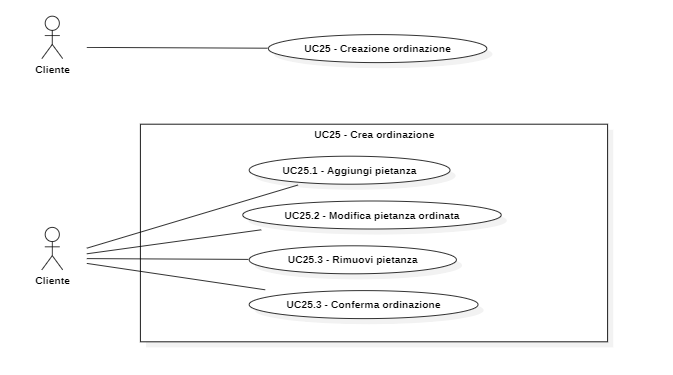
\includegraphics[scale=.8]{uc25.png} \end{figure}
\begin{itemize}
\item \textbf{Attore principale:} Cliente;
\item \textbf{Precondizioni:}
\begin{itemize}
    \item Il cliente ha effettuato una prenotazione (si veda UC19);
    \item Il cliente è nella sezione di riepilogo di una prenotazione singola (si veda UC22);
    \item Il cliente può effettuare l'operazione fino a 48 ore prima dell'orario di prenotazione.
\end{itemize}
\item \textbf{Postcondizioni:} Il cliente ha ordinato le pietanze relative alla prenotazione;
\item \textbf{Scenario principale:}
\begin{enumerate}
    \item Il cliente visualizza la o le sue eventuali ordinazioni confermate precedentemente, oltre a quelle confermate da altri utenti facenti parte della prenotazione;
    \item Il cliente può aggiungere una pietanza al proprio ordine (si veda UC25.1);
    \item Il cliente può modificare una pietanza già aggiunta al proprio ordine (si veda UC25.2);
    \item Il cliente può rimuovere una pietanza dal proprio ordine (si veda UC25.3);
    \item Il cliente conferma la sua ordinazione (si veda UC25.4);
    \item Il sistema aggiorna le informazioni sull'ordinazione del cliente.
\end{enumerate}
\end{itemize}

\pagebreak
\textbf{UC25.1-Aggiungi pietanza/e}
\begin{itemize}
\item \textbf{Attore principale:} Cliente;
\item \textbf{Precondizioni:} Il cliente sta effettuando un'ordinazione (si veda UC25);
\item \textbf{Postcondizioni:} Il cliente ha aggiunto una o più pietanze alla propria ordinazione;
\item \textbf{Scenario principale:}
\begin{enumerate}
    \item Il cliente vede la lista delle pietanze del ristorante presso il quale sta effettuando l'ordinazione;
    \item Il cliente può visualizzare il dettaglio di una singola pietanza (UC25.1.1);
    \item Il cliente può fare una ricerca tra le pietanze (si veda UC25.1.2);
    \item Il cliente dopo aver selezionato una o più pietanze conferma;
    \item Il sistema aggiorna le informazioni sull'ordinazione del cliente.
\end{enumerate}
\end{itemize}

\textbf{UC25.1.1-Visualizza pietanza singola}
\begin{itemize}
\item \textbf{Attore principale:} Cliente;
\item \textbf{Precondizioni:} Il cliente sta visualizzando la lista delle pietanza (si veda UC25.1);
\item \textbf{Postcondizioni:} Il cliente visualizza il dettaglio di una singola pietanza del menù;
\item \textbf{Scenario principale:}
\begin{enumerate}
    \item Il cliente seleziona una pietanza del menù;
    \item Il cliente visualizza il dettaglio di una pietanza ovvero le seguenti informazioni:
    \begin{itemize}
        \item Il nome della pietanza;
        \item Gli ingredienti che compongono la pietanza;
        \item Gli eventuali allergeni contenuti nella pietanza;
        \item Il prezzo della pietanza.
    \end{itemize}
\end{enumerate}
\end{itemize}

\textbf{UC25.1.2-Ricerca pietanza}
\begin{itemize}
\item \textbf{Attore principale:} Cliente;
\item \textbf{Precondizioni:} Il cliente sta visualizzando la lista delle pietanza (si veda UC25.1);
\item \textbf{Postcondizioni:} Il cliente visualizza la lista delle pietanze corrispondenti ai criteri da lui inseriti;
\item \textbf{Scenario principale:}
\begin{enumerate}
    \item Il cliente seleziona la funzionalità di ricerca delle pietanze;
    \item Il cliente può effettuare la ricerca inserendo uno o più parametri, corrispondenti ai seguenti criteri:
    \begin{itemize}
        \item Il nome della pietanza (si veda UC25.1.2.1);
        \item Allergeni non contenuti all'interno della pietanza (si veda UC25.1.2.2).
    \end{itemize}
    \item Il sistema filtra la lista di pietanze secondo i criteri inseriti;
    \item Il cliente visualizza la lista di pietanze che rispettano i criteri da lui inseriti.
\end{enumerate}
\end{itemize}

\textbf{UC25.1.2.1-Ricerca pietanza per nome}
\begin{itemize}
\item \textbf{Attore principale:} Cliente;
\item \textbf{Precondizioni:} Il cliente sta visualizzando la lista delle pietanza (si veda UC25.1);
\item \textbf{Postcondizioni:} Il cliente visualizza la lista delle pietanze corrispondenti alla ricerca per nome da lui inserito;
\item \textbf{Scenario principale:}
\begin{enumerate}
    \item Il cliente seleziona la funzionalità di ricerca di una pietanza;
    \item Il cliente inserisce il testo che deve essere contenuto nel nome;
    \item Il sistema filtra la lista di pietanze secondo il nome inserito;
    \item Il cliente visualizza la lista di pietanze corrispondenti al testo da lui inserito.
\end{enumerate}
\end{itemize}

\textbf{UC25.1.2.1-Ricerca pietanza per allergeni}
\begin{itemize}
\item \textbf{Attore principale:} Cliente;
\item \textbf{Precondizioni:} Il cliente sta visualizzando la lista delle pietanza (si veda UC25.1);
\item \textbf{Postcondizioni:} Il cliente visualizza la lista delle pietanze non contenenti gli allergeni da lui selezionati;
\item \textbf{Scenario principale:}
\begin{enumerate}
    \item Il cliente seleziona la funzionalità di ricerca di una pietanza;
    \item Il cliente seleziona gli allergeni, di default sono selezionati gli allergeni da lui indicati in fase di creazione del profilo (si veda UC6);
    \item Il sistema filtra la lista di pietanze escludendo quelle che contengono gli allergeni selezionati;
    \item Il cliente visualizza la lista di pietanze non contenenti gli allergeni da lui selezionati.
\end{enumerate}
\end{itemize}

\textbf{UC25.2-Modifica pietanza ordinata}
\begin{itemize}
\item \textbf{Attore principale:} Cliente;
\item \textbf{Precondizioni:}
\begin{itemize}
    \item Il cliente sta effettuando un'ordinazione (si veda UC25);
    \item Il cliente ha aggiunto una o più pietanze alla propria ordinazione (si veda UC25.1).
\end{itemize}
\item \textbf{Postcondizioni:} Il cliente ha modificato una pietanza;
\item \textbf{Scenario principale:}
\begin{enumerate}
    \item Il cliente vede la lista delle pietanze da lui ordinate (si veda UC25.1);
    \item Il cliente seleziona l'opzione di modifica di una pietanza;
    \item Il cliente può effettuare le seguenti operazioni di modifica:
    \begin{itemize}
        \item Modificare la quantità della pietanza ordinata (si veda UC25.2.1);
        \item Rimuovere la pietanza ordinata (si veda UC25.2.2);
        \item Aggiungere un ingrediente alla pietanza (si veda UC25.2.3);
        \item Rimuovere un ingrediente dalla pietanza (si veda UC25.2.4).
    \end{itemize}
    \item Il cliente dopo aver modificato la pietanza conferma le sue modifiche;
    \item Il sistema aggiorna le informazioni sulle pietanza dell'ordinazione del cliente;
    \item Il cliente viene reindirizzato alla schermata di creazione ordinazione con le modifiche effettuate alla pietanza (si veda UC25).
\end{enumerate}
\end{itemize}

\textbf{UC25.2.1-Modifica quantità pietanza}
\begin{itemize}
\item \textbf{Attore principale:} Cliente;
\item \textbf{Precondizioni:}
\begin{itemize}
    \item Il cliente sta effettuando un'ordinazione (si veda UC25);
    \item Il cliente sta effettuando una modifica ad una pietanza ordinata (si veda UC25.2).
\end{itemize}
\item \textbf{Postcondizioni:} Il cliente ha modificato la quantità di una pietanza;
\item \textbf{Scenario principale:}
\begin{enumerate}
    \item Il cliente modifica la quantità della pietanza già ordinata, questa non può essere minore di 1;
    \item Il cliente dopo aver modificato la quantità della pietanza conferma le modifiche;
    \item Il sistema aggiorna le informazioni sull'ordinazione del cliente;
    \item Il cliente viene reindirizzato alla schermata di modifica pietanza ordinata (si veda UC25.2).
\end{enumerate}
\end{itemize}

\textbf{UC25.2.2-Aggiungi ingrediente}
\begin{itemize}
\item \textbf{Attore principale:} Cliente;
\item \textbf{Precondizioni:}
\begin{itemize}
    \item Il cliente sta effettuando un'ordinazione (si veda UC25);
    \item Il cliente sta effettuando una modifica ad una pietanza ordinata (si veda UC25.2).
\end{itemize}
\item \textbf{Postcondizioni:} Il cliente ha aggiunto uno o più ingredienti ad una pietanza;
\item \textbf{Scenario principale:}
\begin{enumerate}
    \item Il cliente seleziona l'opzione di aggiunta ingredienti della pietanza;
    \item Il cliente seleziona gli ingredienti che desidera aggiungere alla pietanza dalla lista definita dal ristoratore (si veda UC38);
    \item Il cliente conferma le aggiunte di ingredienti alla pietanza;
    \item Il sistema aggiorna le informazioni sull'ordinazione del cliente;
    \item Il cliente viene reindirizzato alla schermata di modifica pietanza ordinata (si veda UC25.2).
\end{enumerate}
\end{itemize}

\pagebreak
\textbf{UC25.2.3-Rimuovi ingrediente}
\begin{itemize}
\item \textbf{Attore principale:} Cliente;
\item \textbf{Precondizioni:}
\begin{itemize}
    \item Il cliente sta effettuando un'ordinazione (si veda UC25);
    \item Il cliente sta effettuando una modifica ad una pietanza ordinata (si veda UC25.2).
\end{itemize}
\item \textbf{Postcondizioni:} Il cliente ha rimosso uno o più ingredienti da una pietanza;
\item \textbf{Scenario principale:}
\begin{enumerate}
    \item Il cliente seleziona l'opzione di rimozione ingredienti dalla pietanza;
    \item Il cliente seleziona gli ingredienti che desidera rimuovere dalla pietanza;
    \item Il cliente conferma la rimozione degli ingredienti;
    \item Il sistema aggiorna le informazioni sull'ordinazione del cliente;
    \item Il cliente viene reindirizzato alla schermata di modifica pietanza ordinata (si veda UC25.2).
\end{enumerate}
\end{itemize}

\textbf{UC25.3-Rimuovi pietanza}
\begin{itemize}
\item \textbf{Attore principale:} Cliente;
\item \textbf{Precondizioni:}
\begin{itemize}
    \item Il cliente sta effettuando un'ordinazione (si veda UC25);
    \item Il cliente ha aggiunto una o più pietanze alla propria ordinazione (si veda UC25.1).
\end{itemize}
\item \textbf{Postcondizioni:} Il cliente ha eliminato una pietanza;
\item \textbf{Scenario principale:}
\begin{enumerate}
    \item Il cliente seleziona l'opzione di eliminazione della pietanza;
    \item Il sistema aggiorna le informazioni sull'ordinazione del cliente;
    \item Il cliente viene reindirizzato alla schermata di modifica pietanza ordinata (si veda UC25.2).
\end{enumerate}
\end{itemize}

\textbf{UC25.4-Conferma ordinazione}
\begin{itemize}
\item \textbf{Attore principale:} Cliente;
\item \textbf{Precondizioni:}
    \begin{itemize}
        \item Il cliente sta effettuando un'ordinazione (si veda UC25);
        \item Il cliente ha aggiunto una o più pietanze alla propria ordinazione (si veda UC25.1).
    \end{itemize}
\item \textbf{Postcondizioni:} Il cliente ha confermato la sua ordinazione;
\item \textbf{Scenario principale:}
    \begin{enumerate}
        \item Il cliente seleziona l'opzione di conferma ordinazione;
        \item Il sistema aggiorna lo stato dell'ordinazione a "Confermata";
        \item Il cliente viene reindirizzato alla schermata di riepilogo della prenotazione (si veda UC22).
    \end{enumerate}
\end{itemize}

\pagebreak
\subsubsection{UC26-Annullamento ordinazione}
\begin{figure}[h] 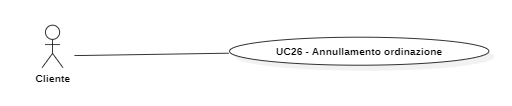
\includegraphics[scale=1]{uc26.png} \end{figure}
\begin{itemize}
\item \textbf{Attore principale:} Cliente;
\item \textbf{Precondizioni:}
\begin{itemize}
    \item Il cliente ha confermato un'ordinazione (si veda UC25.3);
    \item Il cliente può effettuare l'operazione fino a 48 ore prima dell'orario di prenotazione.
\end{itemize}
\item \textbf{Postcondizioni:} L'ordinazione selezionata è stata annullata;
\item \textbf{Scenario principale:}
\begin{enumerate}
    \item Il cliente seleziona l'opzione di annullamento dell'ordinazione;
    \item Il sistema aggiorna le informazioni sull'ordinazione del cliente;
    \item Il cliente viene reindirizzato alla pagina di riepilogo prenotazione priva dell'ordinazione cancellata (si veda UC22).
\end{enumerate}
\end{itemize}
